\documentclass[
11pt, % The default document font size, options: 10pt, 11pt, 12pt
%codirector, % Uncomment to add a codirector to the title page
]{charter} 




% El títulos de la memoria, se usa en la carátula y se puede usar el cualquier lugar del documento con el comando \ttitle
\titulo{Sistema de monitoreo para equipos de captura de CO$_2$} 

% Nombre del posgrado, se usa en la carátula y se puede usar el cualquier lugar del documento con el comando \degreename
%\posgrado{Carrera de Especialización en Sistemas Embebidos} 
\posgrado{Carrera de Especialización en Internet de las Cosas} 
%\posgrado{Carrera de Especialización en Intelegencia Artificial}
%\posgrado{Maestría en Sistemas Embebidos} 
%\posgrado{Maestría en Internet de las cosas}

% Tu nombre, se puede usar el cualquier lugar del documento con el comando \authorname
\autor{Ing. Alena Grebneva} 

% El nombre del director y co-director, se puede usar el cualquier lugar del documento con el comando \supname y \cosupname y \pertesupname y \pertecosupname
\director{Mg. Ing. Milton Eduardo Sosa}
\pertenenciaDirector{FIUBA} 
% FIXME:NO IMPLEMENTADO EL CODIRECTOR ni su pertenencia
\codirector{John Doe} % para que aparezca en la portada se debe descomentar la opción codirector en el documentclass
\pertenenciaCoDirector{FIUBA}

% Nombre del cliente, quien va a aprobar los resultados del proyecto, se puede usar con el comando \clientename y \empclientename
\cliente{Mg. Ing. Eddie Jose Sierra Higuerey}
\empresaCliente{Green Backbone}

% Nombre y pertenencia de los jurados, se pueden usar el cualquier lugar del documento con el comando \jurunoname, \jurdosname y \jurtresname y \perteunoname, \pertedosname y \pertetresname.
\juradoUno{Nombre y Apellido (1)}
\pertenenciaJurUno{pertenencia (1)} 
\juradoDos{Nombre y Apellido (2)}
\pertenenciaJurDos{pertenencia (2)}
\juradoTres{Nombre y Apellido (3)}
\pertenenciaJurTres{pertenencia (3)}
 
\fechaINICIO{25 de abril de 2023}		%Fecha de inicio de la cursada de GdP \fechaInicioName
\fechaFINALPlan{13 de junio de 2023} 	%Fecha de final de cursada de GdP
\fechaFINALTrabajo{Diciembre de 2023}	%Fecha de defensa pública del trabajo final


\begin{document}

\maketitle
\thispagestyle{empty}
\pagebreak


\thispagestyle{empty}
{\setlength{\parskip}{0pt}
\tableofcontents{}
}
\pagebreak


\section*{Registros de cambios}
\label{sec:registro}


\begin{table}[ht]
\label{tab:registro}
\centering
\begin{tabularx}{\linewidth}{@{}|c|X|c|@{}}
\hline
\rowcolor[HTML]{C0C0C0} 
Revisión & \multicolumn{1}{c|}{\cellcolor[HTML]{C0C0C0}Detalles de los cambios realizados} & Fecha      \\ \hline
0      & Creación del documento y asignación del director		&\fechaInicioName \\ \hline
1      & Se completa hasta el punto 5 inclusive             	& 8 de mayo de 2023 \\ \hline
2      & Se completa hasta el punto 9 inclusive				    & 16 de mayo de 2023 \\ \hline
3      & Se completa hasta el punto 12 inclusive                & 23 de mayo de 2023 \\ \hline
4      & Se completa el plan	                                & 30 de mayo de 2023 \\ \hline
\end{tabularx}
\end{table}

\pagebreak



\section*{Acta de constitución del proyecto}
\label{sec:acta}

\begin{flushright}
Buenos Aires, \fechaInicioName
\end{flushright}

\vspace{1cm}

Por medio de la presente se acuerda con la \authorname\hspace{1px} que su Trabajo Final de la \degreename\hspace{1px} se titulará ``\ttitle'' y consistirá en el desarrollo de un prototipo para un sistema capaz de monitorear a distancia los equipos de captura de CO$_2$ pertenecientes al proyecto \textit{Green Backbone}, y tendrá un presupuesto preliminar estimado de 671 h de trabajo y \$ 4.006.755, con fecha de inicio el \fechaInicioName\hspace{1px} y fecha de presentación pública en \fechaFinalName.

Se adjunta a esta acta la planificación inicial.

\vfill

% Esta parte se construye sola con la información que hayan cargado en el preámbulo del documento y no debe modificarla
\begin{table}[ht]
\centering
\begin{tabular}{ccc}
\begin{tabular}[c]{@{}c@{}}Dr. Ing. Ariel Lutenberg \\ Director posgrado FIUBA\end{tabular} & \hspace{2cm} & \begin{tabular}[c]{@{}c@{}}\clientename \\ Fundador de \textit{\empclientename} \end{tabular} \vspace{2.5cm} \\ 
\multicolumn{3}{c}{\begin{tabular}[c]{@{}c@{}} \supname \\ Director del Trabajo Final\end{tabular}} \vspace{2.5cm} \\
%\begin{tabular}[c]{@{}c@{}}\jurunoname \\ Jurado del Trabajo Final\end{tabular}     &  & \begin{tabular}[c]{@{}c@{}}\jurdosname\\ Jurado del Trabajo Final\end{tabular}  \vspace{2.5cm}  \\
%\multicolumn{3}{c}{\begin{tabular}[c]{@{}c@{}} \jurtresname\\ Jurado del Trabajo Final\end{tabular}} \vspace{.5cm}                                                                     
\end{tabular}
\end{table}




\section{1. Descripción técnica-conceptual del proyecto a realizar}
\label{sec:descripcion}
El presente proyecto forma parte de la iniciativa de sostenibilidad \textit{Green Backbone} (en adelante GB). El objetivo de esta iniciativa es hacer frente a los efectos de la emisión de gases de efecto invernadero (GEI) y descarbonizar el aire del ambiente. 

La emisión de GEI que se produce en actividades humanas, tales como la quema de hidrocarburos y la industrialización, se asocia con el cambio climático. Estas emisiones tienen efectos perjudiciales en los sistemas naturales y en los seres humanos a nivel mundial. 

Algunos de los efectos del cambio climático son: el aumento del nivel del mar, el derretimiento de glaciares y la alteración de los patrones climáticos. Estos cambios, a su vez, pueden tener un impacto negativo sobre la seguridad alimentaria, la disponibilidad de agua y la salud de las personas. 

Para hacer frente a esta problemática algunos actores globales (países, compañías e instituciones) se comprometieron a implementar una serie de estrategias que, en primer lugar, permitan reducir gradualmente la emisión de los GEI hacia el año 2030 y luego alcanzar lo que se conoce como \textit{net zero} o emisión cero para el año 2050. 

El concepto de \textit{net zero} o neutralidad de carbono implica lograr un equilibrio entre las emisiones de GEI producidas y las emisiones que se eliminan o se compensan. Por ello, en los últimos años, han surgido iniciativas para el desarrollo de soluciones tecnológicas que permitan remover grandes cantidades de dióxido de carbono (entre 100 y 1.000 Gt de CO$_2$) presente en la atmósfera y alcanzar el \textit{net zero} más rápidamente.

El proyecto GB es liderado el Mg. Ing. Eddie Jose Sierra Higuerey y surgió en Bogotá (Colombia), en el año 2021, como uno de los participantes de la competencia global \textit{XPRIZE Carbon Removal}, donde se ofrecía un premio económico a quienes desarrollen y demuestren la eficiencia de soluciones tecnológicas para secuestrar y retener el dióxido de carbono (CO$_2$) de la atmósfera y los océanos.

Durante la competencia, los miembros del equipo de GB desarrollaron un proceso químico innovador para capturar CO$_2$ del aire y demostraron su funcionamiento en un prototipo de pequeña escala. 

En el proceso químico desarrollado, el aire del ambiente se inyecta con un compresor en un reactor que contiene desechos orgánicos y luego se lo hace circular por un tren de fotobiorreactores. El CO$_2$ queda retenido en ambas etapas del proceso y se puede comercializar como materia prima.

Para capturar grandes volúmenes de CO$_2$ mediante la implementación a gran escala del proceso desarrollado, el equipo de GB de Bogotá comenzó a construir en el año 2022 un prototipo comercial al que se denominó “GB005 Unidad Ángel”. 

Se estima que la unidad GB005 podrá capturar 3,3 toneladas de CO$_2$ al año. También permitirá validar las tecnologías, mejorar el diseño y atraer inversionistas al proyecto.

Para para esta unidad se solicitó a la autora del proyecto desarrollar un dispositivo que registre los niveles de concentración de CO$_2$ en la entrada y la salida de aire del equipo y los muestre en un display LCD, para evaluar el rendimiento del proceso de captura. 

En la figura \ref{fig:diagNodo} se muestra el diagrama en bloques del dispositivo, denominado nodo de medición, al que se adicionaron sensores de temperatura y pH para monitorear la salud de los biorreactores. También se propuso emplear un sensor de luz y relés para controlar el encendido y apagado de la unidad. 

\begin{figure}[htpb]
\centering 
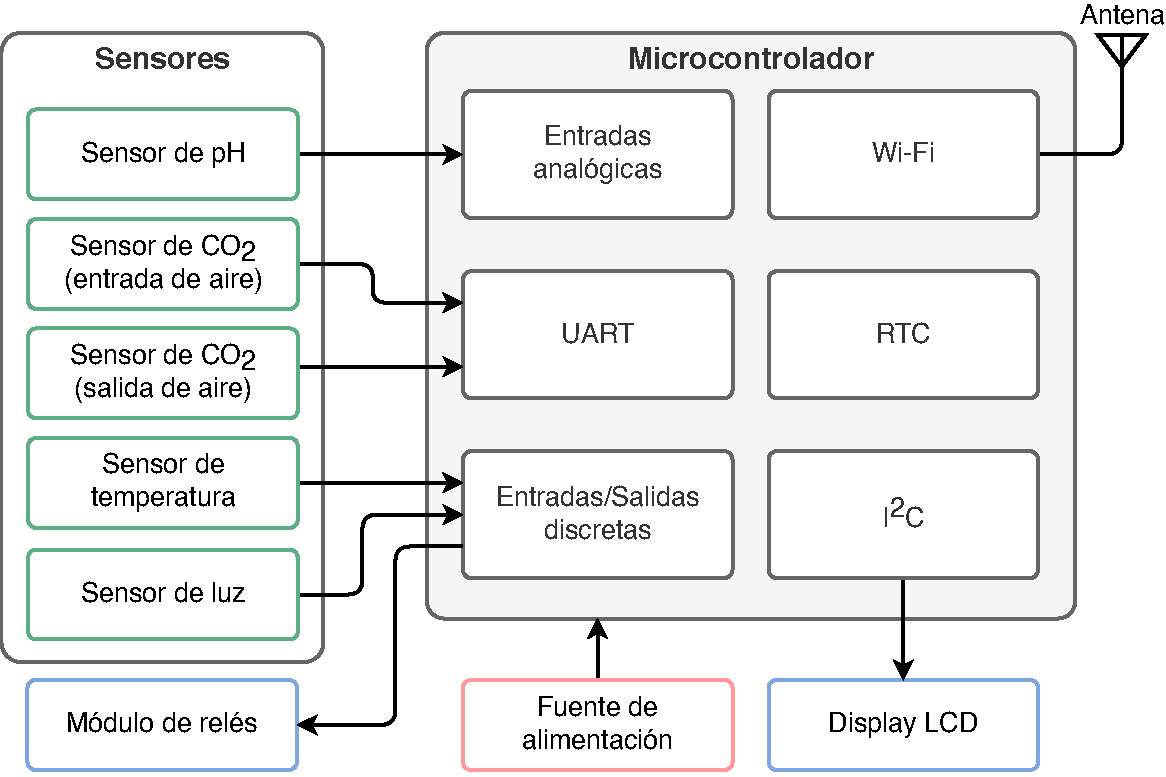
\includegraphics[width=.65\textwidth]{./Figuras/dgNodo.pdf}
\caption{Diagrama en bloques del nodo de medición.}
\label{fig:diagNodo}
\end{figure}

En una instancia de trabajo anterior al curso del posgrado se definió qué microcontrolador y sensores se van a utilizar y se propuso la conexión de todos los elementos. Asimismo, se desarrolló un firmware básico para poder monitorear los niveles de CO$_2$ y mostrar las mediciones en un display. En el presente proyecto se tomará esta base de diseño para mejorar el firmware propuesto.

A futuro, cuando se logre un diseño eficiente y se obtenga financiación, GB proyecta la construcción en serie de nuevas unidades en diferentes tamaños y capacidades de captura. Estas unidades se van a comercializar en Colombia y en el resto del mundo. Por ello, además del nodo de monitoreo para cada unidad, se necesita una plataforma capaz de recolectar y almacenar datos operativos de todas las unidades instaladas, sin importar donde se localicen físicamente.

Como la primera unidad de GB aún se encuentra en etapa de desarrollo, la propuesta del presente proyecto es un prototipo para evaluar su desempeño, agregar funciones de comunicación inalámbrica al nodo para que envíe las mediciones de los sensores hacia un broker MQTT (\textit{Message Queues Telemetry Transport}) y desarrollar la infraestructura del sistema de monitoreo.

En la figura \ref{fig:diagBloques} se muestra una arquitectura tentativa del sistema, que se compone de tres elementos principales: el nodo de medición, un broker MQTT y un entorno de desarrollo para la aplicación de monitoreo.

\begin{figure}[htpb]
\centering 
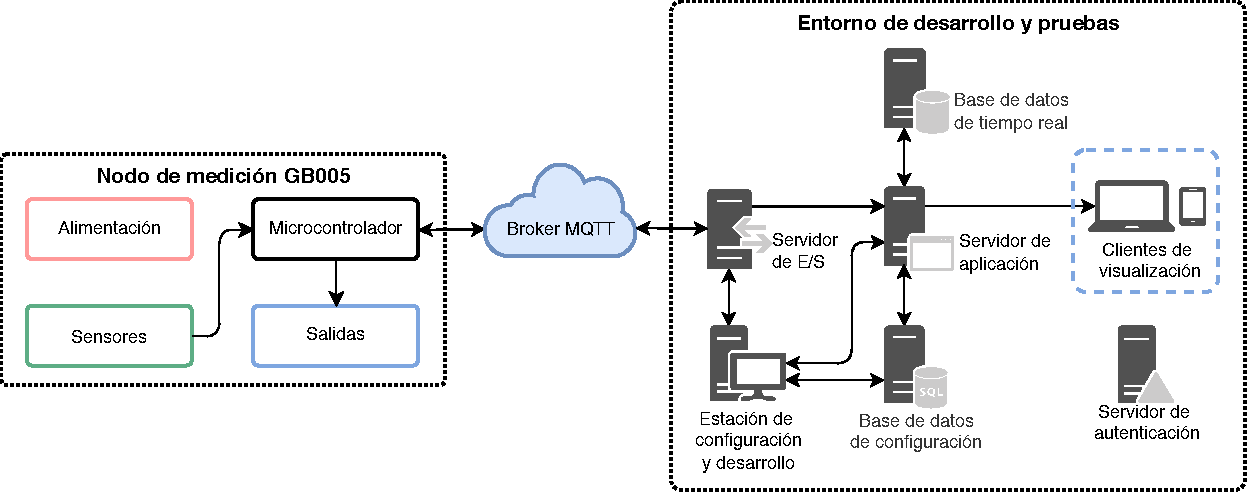
\includegraphics[width=1\textwidth]{./Figuras/diagBloques.pdf}
\caption{Arquitectura del sistema.}
\label{fig:diagBloques}
\end{figure}

El nodo de medición recolecta las mediciones de los sensores y los envía al broker MQTT, que actúa como un intermediario entre el nodo de medición y la aplicación.

La aplicación lee los datos del broker MQTT a través del servidor de entradas y salidas. Utilizando esta información, permite visualizar el funcionamiento general de la unidad en tiempo real a través del servidor de aplicación.

Además de la visualización en tiempo real, la aplicación también almacena la información operativa en una base de datos de tiempo real. Esto permite acceder a los datos históricos y realizar análisis posteriores sobre el funcionamiento de la unidad.

Actualmente existen diferentes soluciones de mercado para implementar aplicaciones IoT. En el presente proyecto, para desarrollar el sistema de monitoreo, se empleará el software \textit{AVEVA System Platform} (ASP) ya que es una solución ampliamente utilizada en la industria con continuo desarrollo y soporte.

El ASP soporta arquitecturas de IoT mediante el uso del protocolo MQTT, posee un entorno gráfico que permite implementar aplicaciones de visualización y una base de datos histórica para almacenar las mediciones de los sensores. 

Además, se tiene acceso a una licencia de desarrollo del ASP sin cargo, ya que la autora del presente proyecto es empleada de AVEVA, la empresa que comercializa la solución. Esto permite reducir costos y tiempos de desarrollo del proyecto.

\section{2. Identificación y análisis de los interesados}
\label{sec:interesados}

\begin{table}[ht]
%\caption{Identificación de los interesados}
%\label{tab:interesados}
\begin{tabularx}{\linewidth}{|l|>{\raggedright\arraybackslash}X|>{\raggedright\arraybackslash}X|l|}
\hline
\rowcolor[HTML]{C0C0C0} 
Rol           & Nombre y Apellido & Organización 		& Puesto 	\\ \hline
%Auspiciante  & -                 & 			 		& -      	\\ \hline
Cliente       & \clientename      &Green Backbone y AVEVA	&  Fundador de GB \\ \hline
%Impulsor     &                   &              		&        	\\ \hline
Responsable   & \authorname       & FIUBA   			& Alumna 	\\ \hline
Colaboradores & -                 & -            		& Empleados de GB/AVEVA \\ \hline
Orientador    & \supname	      	 & \pertesupname 		& Director del trabajo final \\ \hline
%Equipo       & miembro1 \newline 
%				miembro2        	 &              		&        	\\ \hline
%Opositores   &                   &              		&        	\\ \hline
Usuario final & -				 & -            		&  Equipo de GB y sus clientes\\ \hline
\end{tabularx}
\end{table}
\begin{itemize}
	\item Cliente: Eddie Sierra, creó GB como emprendimiento personal y es el principal interesado en el desarrollo de la aplicación de monitoreo para mostrar el valor del proyecto. Trabaja en AVEVA y está impulsando la visibilidad del proyecto GB dentro de esta organización y empresas asociadas para conseguir financiamiento e interesados. Actualmente se ocupa de todas las cuestiones constructivas de la unidad Ángel, con lo cual no dispone de tiempo para hacer un seguimiento detallado del desarrollo. Su prioridad es que el desarrollo tenga el menor costo posible y esté en funcionamiento cuanto antes. Vive en Colombia y se debe considerar la diferencia horaria para programar reuniones con él.
	\item Orientador: Milton Sosa, ayudará con la definición de los requerimientos y alcance del proyecto. Se encuentra viviendo en Europa y se debe considerar la diferencia horaria para programar reuniones con él.
	\item Usuario final: los miembros del equipo de GB y sus clientes utilizarán la plataforma desde diferentes partes del mundo para visualizar el estado de funcionamiento y rendimiento de las unidades.
\end{itemize}


\section{3. Propósito del proyecto}
\label{sec:proposito}

Desarrollar e implementar el prototipo para una plataforma de monitoreo que permita visualizar en tiempo real y almacenar el historial de los datos operacionales de la unidad GB005 y las unidades futuras del proyecto \textit{Green Backbone}. 

El objetivo de este prototipo será monitorear el estado de funcionamiento de las unidades, evaluar su rendimiento y poder programar el mantenimiento o recambio de consumibles.

\section{4. Alcance del proyecto}
\label{sec:alcance}
El proyecto incluye:
\begin{itemize}
	\item Adaptación del firmware del nodo para que envíe datos mediante el protocolo MQTT
	\item Despliegue y configuración del entorno de desarrollo y pruebas
		\begin{itemize}
		\item Configuración del entorno virtual
		\item Instalación y licenciamiento del software ASP
		\item Configuración de acceso y seguridad
		\end{itemize}
	\item Configuración de la colección e historización de datos
	\item Desarrollo de la aplicación de visualización en tiempo real
	\item Desarrollo de plantillas para las unidades futuras
	
\end{itemize}

El proyecto no incluye:
\begin{itemize}
	\item Desarrollo del hardware del nodo de medición
	\item Despliegue del broker MQTT
	\item Contratación de servicios en la nube para implementar la aplicación de monitoreo
	\item Adquisición de cualquier otra licencia de software que pueda ser requerida
	\item Puesta en marcha para producción
	
\end{itemize}

\section{5. Supuestos del proyecto}
\label{sec:supuestos}

Para el desarrollo del presente proyecto se supone que: 
\begin{itemize}
	\item Se contará con los recursos económicos necesarios para realizar del proyecto.
	\item Se tendrá a disposición la infraestructura de hardware necesaria para implementar la aplicación de monitoreo.
	\item Se dispondrá una conexión a Internet mediante Wi-Fi continuamente para las pruebas.
	\item No habrá dificultades para conseguir el software necesario (licencias, bibliotecas, certificaciones, etc).
	\item Se dispondrá del conocimiento necesario para programar el microcontrolador.
	\item Se dispondrá del conocimiento para desarrollar la aplicación de monitoreo.
	\item Se contará con la colaboración de profesionales idóneos en temas de conectividad, programación del microcontrolador y desarrollo de aplicaciones con el ASP.
	\item El cliente aceptará que algunas mediciones sean simuladas por no disponer de los sensores localmente.
\end{itemize}

\section{6. Requerimientos}
\label{sec:requerimientos}

\begin{enumerate}
	\item Requerimientos de \textit{firmware} del nodo de medición
		\begin{enumerate}
                \item Correr sobre un microcontrolador ESP32 (ESP-WROOM-32)
			\item Disponer de conexión a una red Wi-Fi en el sitio para pruebas
			\item Envío y recepción de datos mediante el protocolo MQTT, utilizando certificados SSL/TLS para la comunicación con el broker
			\item Obtención de información horaria desde un servidor NTP
			\item Lectura de las mediciones de CO$_2$ de dos sensores MH-Z19B/T6793 empleando los puertos UART/I$^2$C
               \begin{itemize}
                   \item Los sensores MH-Z19B poseen un rango de medición entre 0 y 5000 ppm con una precisión de ±50 ppm y salida UART TTL de 3.3 V.
                   \item Los sensores T6793 poseen un rango de medición entre 0 y 2000 ppm con una precisión de ±45 ppm y salida I$^2$C que soporta Modbus.
               \end{itemize}
			\item Lectura de la medición de temperatura de un sensor digital DS18B20, utilizando el protocolo \textit{1-Wire}
                \begin{itemize}
                   \item Este sensor posee un rango de medición entre -55°C y 125°C con una precisión de ±0.5°C entre -10 y +85 °C, tiene una resolución programable entre 9 y 12 bits y cuenta con una salida digital de datos para la comunicación bidireccional con el microcontrolador.
               \end{itemize}
			\item Lectura y conversión de la medición del pH de un sensor SEN0249, mediante el ADC del microcontrolador
                \begin{itemize}
                   \item Este sensor posee un rango de medición entre 0 y 14 pH, tiene una precisión de ±0.1 pH y cuenta con un transmisor con salida analógica entre 0 y 3.3 V.
               \end{itemize}
			\item Detección de luz diurna a través de un módulo fotorresistivo LDR (\textit{Light Depending Resistor}) conectado a una entrada discreta
                \begin{itemize}
                   \item Este sensor posee una salida discreta que indica con un nivel alto que la intensidad de la luz se encuentra por debajo de cierto umbral (que se establece mediante el potenciómetro de la placa).
               \end{itemize}
			\item Accionamiento de un módulo con relés mediante salidas discretas, para encender y apagar los compresores
                \begin{itemize}
                   \item Este módulo posee dos entradas opto-acopladas y dos salidas a relé que permiten controlar la conexión y desconexión de cargas de hasta 250 V (CA) y 10 A.
               \end{itemize}
			\item Visualización de las mediciones en un display LCD1602 conectado al puerto I$^2$C
                \begin{itemize}
                   \item Este display posee 16 caracteres en 2 líneas, color azul con retro-iluminación ajustable e incluye un adaptador para I$^2$C.
               \end{itemize}
   
		\end{enumerate}
	\item Requerimientos funcionales del broker MQTT
		\begin{enumerate}
			\item Proveer certificados SSL/TLS para la comunicación del microcontrolador y la aplicación de monitoreo
			\item Ser capaz de manejar múltiples conexiones simultáneas de nodos de monitoreo
			\item Ser de acceso público
		\end{enumerate}
	\item Requerimientos de la aplicación de monitoreo
		\begin{enumerate}
			\item Envío y recepción de datos mediante el protocolo MQTT, utilizando certificados SSL/TLS para la comunicación con el broker
			\item Organización de los datos recibidos en una estructura jerárquica
			\item Visualización de las mediciones en tiempo real 
			\item Registro de las mediciones obtenidas en una base de datos
			\item Autenticación de los usuarios y control de acceso a las funcionalidades
			\item Escalabilidad para agregar nuevas unidades de GB a futuro
			\item Generación de alarmas cuando se superen los umbrales definidos para las mediciones
			\item Configuración de los umbrales de alarma
			\item Generar reportes de datos instantáneos e históricos
			\item Manejo de errores de comunicación con el broker MQTT y con la base de datos
		\end{enumerate}	
	\item Requerimientos de la interfaz de visualización
		\begin{enumerate}
			\item Mostrar las mediciones de los sensores en tiempo real de manera gráfica
			\item Permitir la visualización de datos históricos
			\item Ser fácil de usar para cualquier usuario sin conocimientos técnicos especializados
			\item Comunicarse con la aplicación de monitoreo mediante un protocolo de comunicación seguro 
			\item Mostrar alertas y notificaciones de las alarmas generadas
			\item Ser accesible desde cualquier dispositivo con conexión a Internet y compatible con diferentes navegadores
			\item Proteger los datos mediante autenticación y autorización de usuarios
			
		\end{enumerate}	
	\item Requerimientos de \textit{testing}
		\begin{enumerate}
			\item Pruebas de funcionalidad para validar que el nodo de monitoreo realice la lectura de las mediciones desde los sensores sin errores, por ejemplo, contrastando los valores medidos contra un sensor calibrado o valores tabulados para las condiciones ambientales bajo las que se realizó una determinada medición.
 			\item Pruebas de comunicación para validar que el broker MQTT recibe los datos enviados por el nodo de medición, por ejemplo, empleando un cliente MQTT externo.
 			\item Pruebas de comunicación para validar que el servidor de entradas/salidas de la aplicación de monitoreo reciba las mediciones del broker MQTT con el mismo formato enviado desde el nodo de medición.
			\item Pruebas de integración para validar que los diferentes componentes del sistema funcionen en conjunto, de modo que en la aplicación de monitoreo y base de datos histórica que se vean exactamente los mismos datos que genera el nodo de medición.
			\item Se deberán realizar pruebas de seguridad para validar que el acceso a las herramientas de desarrollo y visualización solamente sean accesibles para los usuarios autorizados.
		\end{enumerate}	
\end{enumerate}

\section{7. Historias de usuarios (\textit{Product backlog})}
\label{sec:backlog}
Para determinar los \textit{story points} de una historia de usuario, se asignaron valores a cada uno de los siguientes aspectos:
\begin{itemize}
\item Complejidad del trabajo:
	\begin{itemize}
	\item Alta: 13
	\item Media: 5
	\item Baja: 1
	\end{itemize}
\item Dificultad del trabajo:
	\begin{itemize}
	\item Alta: 5
	\item Media: 3
	\item Baja: 1
	\end{itemize}
\item Incertidumbre del trabajo:
	\begin{itemize}
	\item Alta: 5
	\item Media: 3
	\item Baja: 1
	\end{itemize}
\end{itemize}

Para obtener los \textit{story points}, se sumaron los valores asignados a cada aspecto y se aproximaron al siguiente número de la serie de Fibonacci.

Por ejemplo, si la complejidad del trabajo es media (5), la dificultad es alta (5) y la incertidumbre es media (3), los \textit{story points} serían 21 (5 + 5 + 3 = 13, que se aproxima al siguiente número de Fibonacci, que es 21).
\begin{enumerate}
\item Como miembro del equipo de GB, quiero registrar los niveles de concentración de CO$_2$ en la entrada y la salida de aire de la unidad, para evaluar el rendimiento del proceso de captura.
\textit{Story points}: 8 (complejidad: 3, dificultad: 2, incertidumbre: 3)

\item Como miembro del equipo de GB, quiero que la unidad tenga conexión a Internet y envíe los datos de los sensores a una plataforma de monitoreo centralizada.

\textit{Story points}: 13 (complejidad: 5, dificultad: 3, incertidumbre: 5)

\item Como miembro del equipo de GB, quiero acceder a un registro histórico de las lecturas y alarmas generadas por cada unidad, para poder analizar su comportamiento en el largo plazo. 

\textit{Story points}: 8 (complejidad: 3, dificultad: 3, incertidumbre: 1)

\item Como miembro del equipo de GB, quiero que la plataforma de monitoreo sea segura y proteja los datos recolectados por los nodos de medición, para evitar posibles ataques o filtraciones de información. 

\textit{Story points}: 13 (complejidad: 5, dificultad: 5, incertidumbre: 3)

\item Como usuario, quiero ver los datos de funcionamiento y estadísticas sobre el rendimiento de mi unidad, desde una interfaz fácil de usar. 

\textit{Story points}: 13 (complejidad: 5, dificultad: 5, incertidumbre: 2)

\item Como usuario, quiero que el sistema de monitoreo me muestre alarmas cuando se detecten niveles de concentración de CO$_2$ en la entrada o salida de aire por encima o por debajo de ciertos umbrales. 

\textit{Story points}: 8 (complejidad: 2, dificultad: 3, incertidumbre: 3)

\item Como ingeniero de mantenimiento, quiero que el dispositivo registre y muestre en tiempo real la temperatura y el pH de los biorreactores de la unidad, para monitorear su funcionamiento y programar el cambio de consumibles.

\textit{Story points}: 13 (complejidad: 5, dificultad: 5, incertidumbre: 2)

\item Como ingeniero de mantenimiento, quiero que la unidad funcione solo durante las horas del día en que hay luz solar disponible para ahorrar energía y consumibles.

\textit{Story points}: 8 (complejidad: 3, dificultad: 2, incertidumbre: 3)

\item Como ingeniero de desarrollo, quiero garantizar que la plataforma sea escalable para incorporar nuevas unidades, a medida que se expande el negocio de \textit{Green Backbone}. 

\textit{Story points}: 8 (complejidad: 3, dificultad: 2, incertidumbre: 3)

\item Como ingeniero de desarrollo, quiero poder asignar roles y permisos de usuario para garantizar que los datos sean accesibles solo para personas autorizadas. 

\textit{Story points}: 8 (complejidad: 2, dificultad: 5, incertidumbre: 1)

\item Como científico de datos quiero que la plataforma de monitoreo tenga la capacidad de generar informes para poder analizar los datos operativos de manera detallada. 

\textit{Story points}: 13 (complejidad: 5, dificultad: 3, incertidumbre: 3)
\end{enumerate}

\section{8. Entregables principales del proyecto}
\label{sec:entregables}
\begin{itemize}
\item Firmware mejorado para el nodo de medición, que permitirá enviar mediciones de los sensores hacia un broker MQTT y podrá ser utilizado para futuras unidades de GB.

\item Sistema de monitoreo para la unidad GB005, que permitirá visualizar en tiempo real las mediciones de CO$_2$, temperatura, pH y luz, así como el estado de encendido y apagado de la unidad.

\item Plataforma para recolectar y almacenar datos operativos de todas las unidades instaladas de GB, capaz de recibir datos de los nodos de medición mediante un broker MQTT y mostrarlos en una interfaz de usuario.

\item Documentación técnica del proyecto, que incluye diagramas y esquemáticos de conexión, listados de componentes, código fuente del firmware y archivos de backup del sistema de monitoreo.
\end{itemize}
\section{9. Desglose del trabajo en tareas}
\label{sec:wbs}
\begin{enumerate}
	\item Gestión de proyecto (50 h)
	\begin{enumerate}
		\item Reuniones con el cliente y con el director del trabajo (10 h)
		\item Elaboración del plan de proyecto de Trabajo Final (20 h)
		\item Elaboración de la presentación del plan de proyecto (10 h)
		\item Revisión y correcciones de los entregables (10 h)
	\end{enumerate}
	\item Investigación preliminar y aprendizaje de tecnologías (120 h)
	\begin{enumerate}
		\item Protocolos de comunicación (40 h)
		\item Lenguajes de programación (40 h)
		\item Herramientas de desarrollo (40 h)
	\end{enumerate}
		\item Desarrollo del firmware para el microcontrolador (111 h)
	\begin{enumerate}
		\item Portar desarrollo existente en el \textit{framework} Arduino al de ESP-IDF (10 h)
		\item Programación de la conexión Wi-Fi y configuración de la red (5 h)
		\item Implementación del protocolo MQTT con certificados SSL/TLS (20 h)
		\item Integración del servidor NTP para obtener información horaria (2 h)
		\item Programación de la adquisición de mediciones (34 h)
		\begin{enumerate}[label*=\arabic*.,ref=\theenumii.\arabic*]
			\item Definición de conexiones entre el microcontrolador y los sensores (10 h)
			\item Lectura de niveles de CO$_2$ desde los sensores MH-Z19B (5 h)
			\item Lectura de la temperatura del sensor DS18B20 (5 h)
			\item Simulación de la medición del pH (5 h)
			\item Detección de luz diurna (2 h)
			\item Accionamiento de los relés (2 h)
			\item Visualización de las mediciones en el display LCD (5 h)
		\end{enumerate}
		\item Pruebas de adquisición de datos de todos los sensores disponibles (10 h)
		\item Pruebas de envío de mediciones de todos los sensores al broker MQTT (10 h)
		\item Corrección de errores (20 h)
	\end{enumerate}
	\item Desarrollo del \textit{backend} de la aplicación de monitoreo (165 h)
	\begin{enumerate}
		\item Configuración del entorno de desarrollo y pruebas (20 h)
		\item Instalación y licenciamiento del software ASP (10 h)
		\item Configuración de acceso y seguridad en el ASP (15 h)
		\item Modelado de la aplicación mediante objetos (40 h)
		\item Configuración de la adquisición de datos mediante el driver MQTT (20 h)
		\item Configuración de la historización de datos (10 h)
		\item Despliegue del \textit{runtime} de la aplicación (10 h)
		\item Pruebas de adquisición de datos (10 h)
		\item Pruebas de funcionamiento en \textit{runtime} (10 h)
		\item Corrección de errores (20 h)
	\end{enumerate}
	\item Desarrollo del \textit{frontend} de la aplicación de monitoreo (130 h)
	\begin{enumerate}
		\item Diseño del \textit{layout} de la interfaz de usuario (20 h)
		\item Implementación de la visualización de datos en tiempo real (30 h)
		\item Implementación de la visualización de datos históricos (10 h)
		\item Implementación del acceso remoto a la aplicación de visualización (20 h)
		\item Implementación de reportes (20 h)
		\item Pruebas de funcionamiento en \textit{runtime} (10 h)
		\item Corrección de errores (20 h)
	\end{enumerate}
	\item Generación de entregables y proceso de cierre (95 h)
	\begin{enumerate}
		\item Elaboración del informe de avance (15 h)
		\item Elaboración memoria técnica de Trabajo Final (40 h)
		\item Revisión y correcciones de la memoria (15 h)
		\item Elaboración de la presentación final (15 h)
		\item Revisión y correcciones de la presentación final (10h)
	\end{enumerate}
\end{enumerate}

Cantidad total de horas: 671 h.

\section{10. Diagrama de Activity On Node}
\label{sec:AoN}
En la figura \ref{fig:AoN_lt} se muestran los grupos de tareas, junto con el camino crítico.
\begin{figure}[htpb]
\centering 
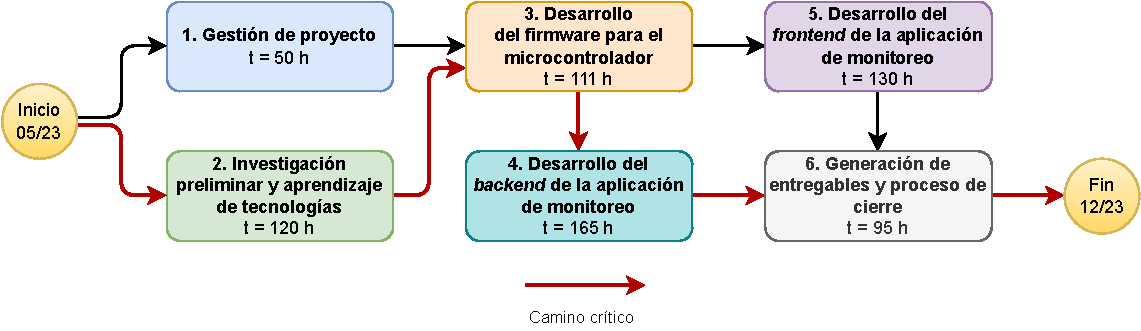
\includegraphics[width=.9\textwidth]{./Figuras/AON_Light.pdf}
\caption{Diagrama de \textit{Activity on Node} de alto nivel.}
\label{fig:AoN_lt}
\end{figure}

En la figura \ref{fig:AoN} se muestra el diagrama de \textit{Activity on Node} con el detalle de todas las tareas del proyecto, también indicando el camino crítico.
\begin{figure}[htpb]
\centering 
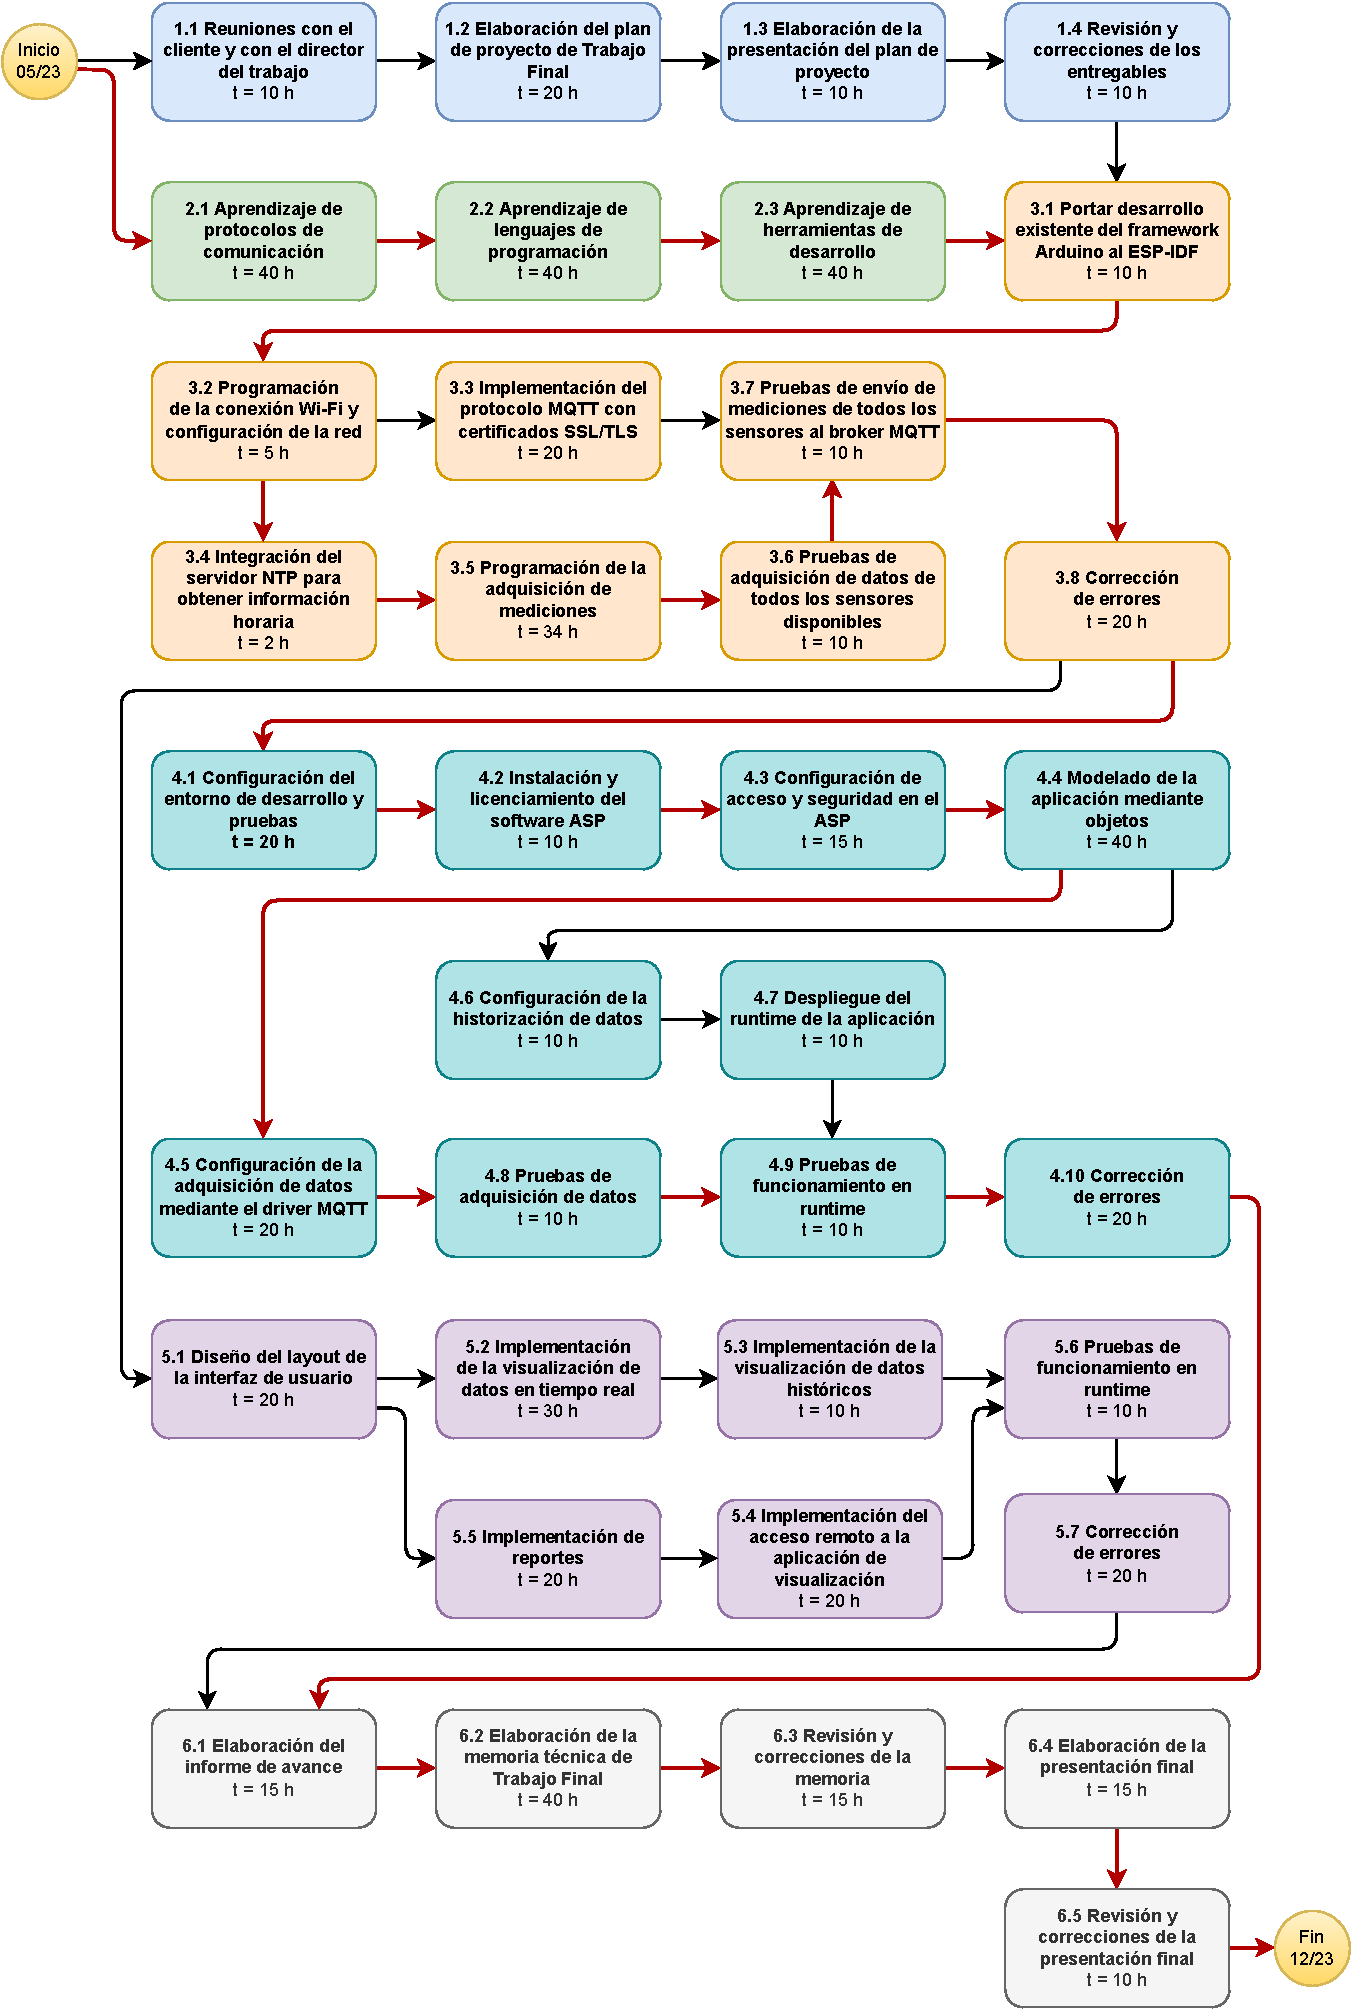
\includegraphics[width=1\textwidth]{./Figuras/AON_Full.pdf}
\caption{Diagrama de \textit{Activity on Node} detallado.}
\label{fig:AoN}
\end{figure}

\pagebreak
\begin{landscape}
\section{11. Diagrama de Gantt}
\label{sec:gantt}

\begin{figure}[htpb]
\centering 
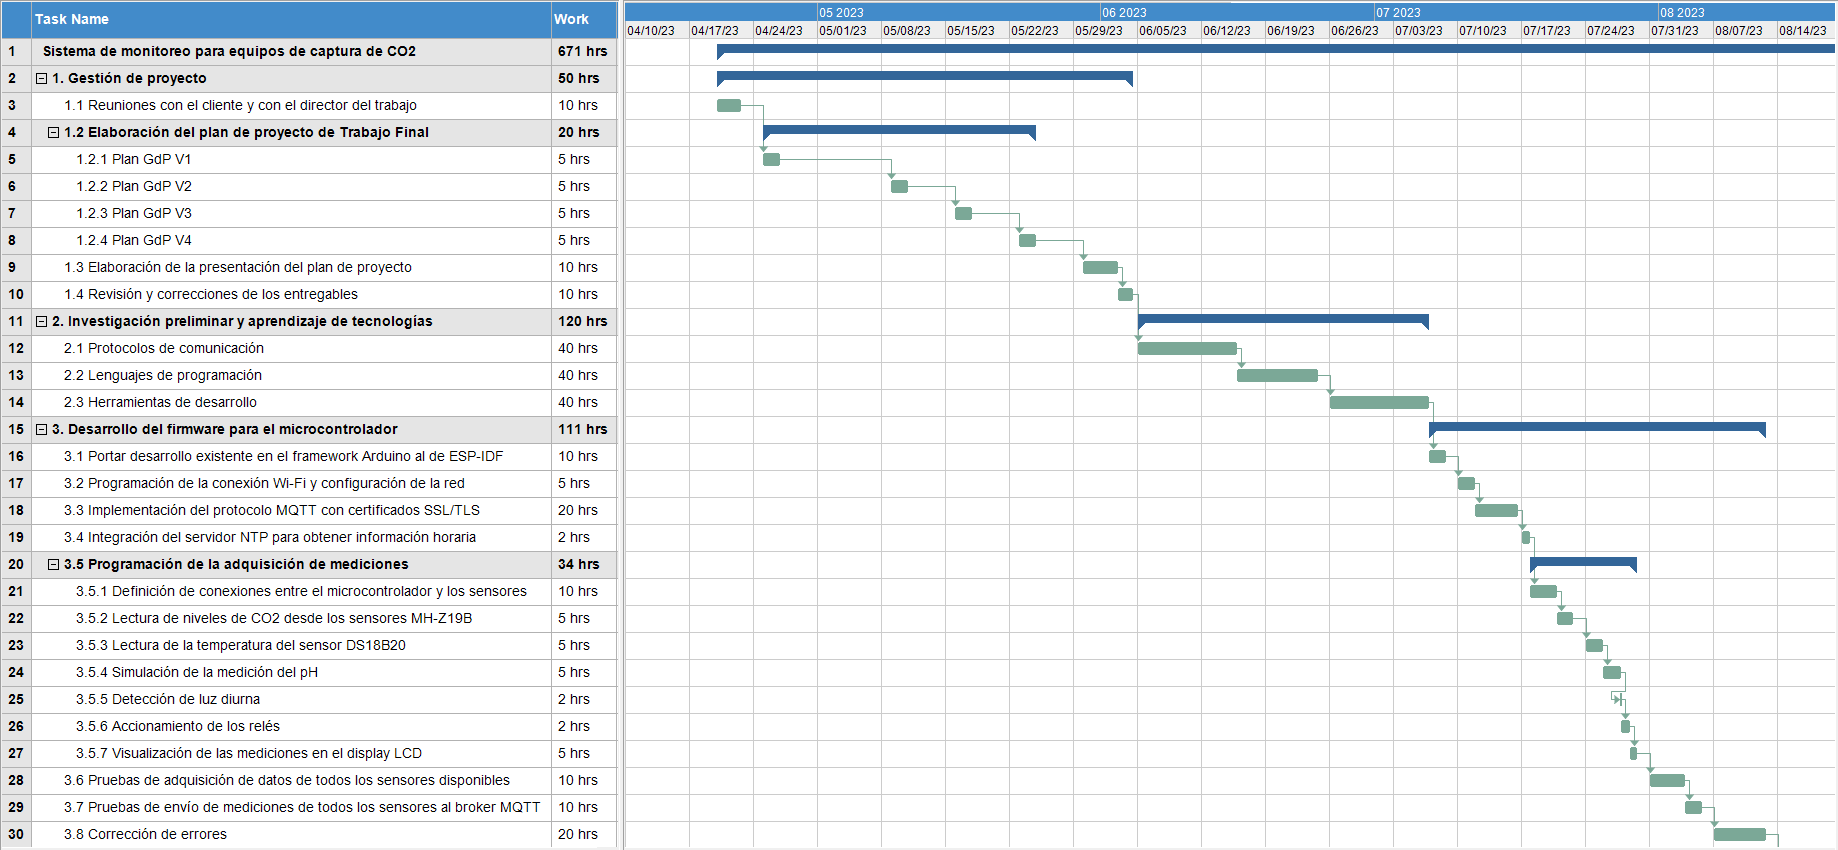
\includegraphics[height=.70\textheight]{./Figuras/Gantt01.png}
\caption{Diagrama de Gantt del proyecto (parte 1).}
\label{fig:diagGantt01}
\end{figure}
\end{landscape}

\begin{landscape}
\begin{figure}[htpb]
\centering 
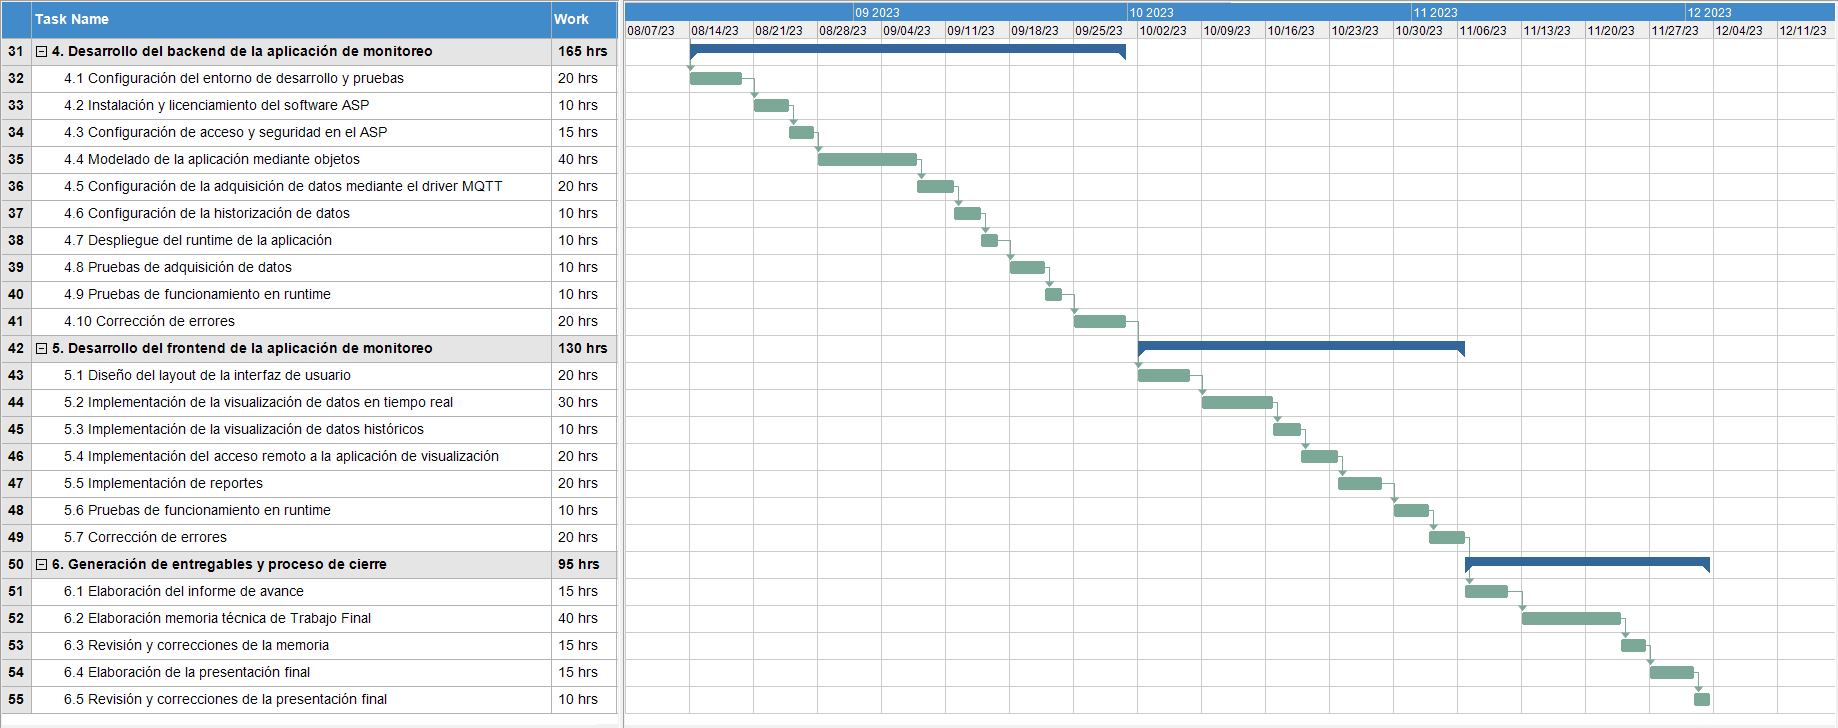
\includegraphics[height=.60\textheight]{./Figuras/Gantt02.png}
\caption{Diagrama de Gantt del proyecto (parte 2).}
\label{fig:diagGantt02}
\end{figure}
\end{landscape}

\section{12. Presupuesto detallado del proyecto}
\label{sec:presupuesto}

A continuación, se muestra el presupuesto del proyecto, expresado en pesos argentinos.

\begin{table}[htpb]
\centering
\begin{tabularx}{\linewidth}{@{}|X|c|r|r|@{}}
\hline
\rowcolor[HTML]{C0C0C0} 
\multicolumn{4}{|c|}{\cellcolor[HTML]{C0C0C0}COSTOS DIRECTOS} \\ \hline
\rowcolor[HTML]{C0C0C0} 
Descripción &
  \multicolumn{1}{c|}{\cellcolor[HTML]{C0C0C0}Cantidad} &
  \multicolumn{1}{c|}{\cellcolor[HTML]{C0C0C0}Valor unitario} &
  \multicolumn{1}{c|}{\cellcolor[HTML]{C0C0C0}Valor total} \\ \hline
% fila 1
  \multicolumn{1}{|l|}{Horas de ingeniería y desarrollo}  &
  \multicolumn{1}{c|}{671} &
  \multicolumn{1}{c|}{\$ 4.000} &
  \multicolumn{1}{c|}{\$ 2.684.000} \\ \hline
% fila 2 
  \multicolumn{1}{|l|}{Microcontrolador ESP32 ESP-WROOM-32 Wi-Fi} &
  \multicolumn{1}{c|}{1} &
  \multicolumn{1}{c|}{\$ 4.000} &
  \multicolumn{1}{c|}{\$ 4.000} \\ \hline
% fila 3 
  \multicolumn{1}{|l|}{Sensor de CO$_2$ NDIR MH-Z19B} &
  \multicolumn{1}{c|}{2} &
  \multicolumn{1}{c|}{\$ 29.950} &
  \multicolumn{1}{c|}{\$ 59.900} \\ \hline
% fila 4 
  \multicolumn{1}{|l|}{Sensor de CO$_2$ NDIR T6793} &
  \multicolumn{1}{c|}{2} &
  \multicolumn{1}{c|}{\$ 19.967} &
  \multicolumn{1}{c|}{\$ 39.934} \\ \hline
% fila 5 
  \multicolumn{1}{|l|}{Sensor de temperatura DS18B20 sumergible} &
  \multicolumn{1}{c|}{1} &
  \multicolumn{1}{c|}{\$ 1.120} &
  \multicolumn{1}{c|}{\$ 1.120} \\ \hline
% fila 6 
  \multicolumn{1}{|l|}{Display LCD 1602 I$^2$C azul} &
  \multicolumn{1}{c|}{1} &
  \multicolumn{1}{c|}{\$ 3.000} &
  \multicolumn{1}{c|}{\$ 3.000} \\ \hline
% fila 7 
  \multicolumn{1}{|l|}{Sensor de pH DFRobot SEN0249} &
  \multicolumn{1}{c|}{1} &
  \multicolumn{1}{c|}{\$ 67.857} &
  \multicolumn{1}{c|}{\$ 67.857} \\ \hline
% fila 8 
  \multicolumn{1}{|l|}{Módulo de relés 2 canales 5 V} &
  \multicolumn{1}{c|}{1} &
  \multicolumn{1}{c|}{\$ 1.525} &
  \multicolumn{1}{c|}{\$ 1.525} \\ \hline
% fila 9 
  \multicolumn{1}{|l|}{Módulo sensor de luz con LDR} &
  \multicolumn{1}{c|}{1} &
  \multicolumn{1}{c|}{\$ 632} &
  \multicolumn{1}{c|}{\$ 632} \\ \hline
\multicolumn{3}{|c|}{SUBTOTAL} &
  \multicolumn{1}{c|}{\$ 2.861.968} \\ \hline
\rowcolor[HTML]{C0C0C0} 
\multicolumn{4}{|c|}{\cellcolor[HTML]{C0C0C0}COSTOS INDIRECTOS} \\ \hline
\rowcolor[HTML]{C0C0C0} 
Descripción &
  \multicolumn{1}{c|}{\cellcolor[HTML]{C0C0C0}Cantidad} &
  \multicolumn{1}{c|}{\cellcolor[HTML]{C0C0C0}Valor unitario} &
  \multicolumn{1}{c|}{\cellcolor[HTML]{C0C0C0}Valor total} \\ \hline
\multicolumn{1}{|l|}{40 \% de los costos directos} &
  \multicolumn{1}{c|}{1} &
  \multicolumn{1}{c|}{\$ 1.144.787} &
  \multicolumn{1}{c|}{\$ 1.144.787} \\ \hline
\multicolumn{3}{|c|}{SUBTOTAL} &
  \multicolumn{1}{c|}{\$ 1.144.787} \\ \hline
\rowcolor[HTML]{C0C0C0}
\multicolumn{3}{|c|}{TOTAL} & \$ 4.006.755
   \\ \hline
\end{tabularx}%
\end{table}


\section{13. Gestión de riesgos}
\label{sec:riesgos}

a) Identificación de los riesgos y estimación de sus consecuencias:

Los riesgos listados a continuación serán cuantificados, en un rango del 1 al 10, en los siguientes índices:
Severidad (S): cuanto más severo el riesgo, más alto el número.
Ocurrencia (O): cuanto más probable es que ocurra el riesgo, más alto el número.

Riesgo 1: falla en la conexión a Internet en el sitio de pruebas.
\begin{itemize}
	\item Severidad (S): 7. Esta falla impediría la comunicación entre el nodo de medición y el broker MQTT, lo que afectaría la visualización de datos en la aplicación de monitoreo.
	\item Probabilidad de ocurrencia (O): 5. La probabilidad puede ser moderada, ya que depende de la calidad y estabilidad, tanto de la red interna, como del proveedor de servicios de internet en el sitio de pruebas. 
\end{itemize}   

Riesgo 2: errores de firmware que afecten el envío de datos al broker MQTT.
\begin{itemize}
	\item Severidad (S): 6. Si hay errores en el firmware del nodo de medición, los datos pueden enviarse incorrectamente o no enviarse en absoluto. Esto dificulta el monitoreo en tiempo real y la obtención de datos.
	\item Ocurrencia (O): 4. Los errores en el firmware pueden ocurrir debido a problemas de programación, falta de pruebas exhaustivas o cambios inesperados en los requisitos. Existe una probabilidad moderada de que se presenten errores en el firmware del nodo de medición.
\end{itemize}

Riesgo 3: falla de los sensores que genere mediciones inexactas o nulas.
\begin{itemize}
	\item Severidad (S): 9. Ante la falla de uno o varios sensores, las mediciones obtenidas podrían ser inexactas o nulas, lo que afectaría la calidad y utilidad de los datos recopilados y visualizados en la plataforma de monitoreo.
	\item Ocurrencia (O): 4. La probabilidad de fallos en los sensores de medición puede ser baja, especialmente si se utilizan sensores de alta calidad y se realiza un mantenimiento adecuado. Sin embargo, existe la posibilidad de que los sensores experimenten problemas técnicos o de calibración.
\end{itemize}

Riesgo 4: errores en la configuración de seguridad y acceso de la plataforma de monitoreo.
\begin{itemize}
	\item Severidad (S): 6. Implica problemas de autenticación y control de acceso a la plataforma de monitoreo, lo que podría comprometer la integridad y privacidad de los datos y la funcionalidad general del sistema.
	\item Ocurrencia (O): 6. La probabilidad puede ser moderada, ya que depende de la precisión y exhaustividad con la que se configuren los mecanismos de seguridad y acceso.
\end{itemize}

Riesgo 5: desvinculación de algún miembro importante del equipo de GB de su trabajo principal.
\begin{itemize}
	\item Severidad (S): 8. Implica que no se tenga más acceso a herramientas o recursos cruciales para el desarrollo de alguna de las partes del proyecto. Esto a su vez deriva en un cambio de alcance o requerimientos con el proyecto en marcha.
	\item Ocurrencia (O): 4. Hay una probabilidad moderada de que algún miembro se desvincule de la compañía, ya sea por una oportunidad de crecimiento profesional en otra compañía o por recorte de costos.
\end{itemize}

Riesgo 6: cambios en los requerimientos del cliente.
\begin{itemize}
	\item Severidad (S): 7. Si se producen cambios significativos en los requerimientos del cliente durante el desarrollo del proyecto, podría ser necesario ajustar el diseño y la implementación, lo que podría generar retrasos y costos adicionales.
	\item Ocurrencia (O): 6. La probabilidad de que se produzcan cambios en los requerimientos del cliente es moderada, ya que es común que surjan nuevas necesidades o se realicen ajustes a medida que avanza el proyecto.
\end{itemize}

b) Tabla de gestión de riesgos, donde el RPN se calcula como RPN=SxO:

\begin{table}[htpb]
\centering
\begin{tabularx}{\linewidth}{@{}|X|c|c|c|c|c|c|@{}}
\hline
\rowcolor[HTML]{C0C0C0}
Riesgo & S & O & RPN & S* & O* & RPN* \\ \hline

Falla en la conexión a Internet en el sitio de pruebas & 7 & 5 & 35 & & & \\ \hline
Errores de firmware que afecten el envío de datos al broker MQTT & 6 & 5 & 30 & & & \\ \hline
Falla de los sensores que genere mediciones inexactas o nulas & 9 & 4 & 36 & 7 & 3 & 21 \\ \hline
Errores en la configuración de seguridad y acceso de la plataforma de monitoreo & 6 & 6 & 36 & 6 & 5 & 30 \\ \hline
Desvinculación de algún miembro importante del equipo de GB de su trabajo principal & 8 & 4 & 32 & & & \\ \hline
Cambios en los requerimientos del cliente & 7 & 6 & 42 & 7 & 4 & 28 \\ \hline
\end{tabularx}%
\end{table}

Criterio adoptado: se tomarán medidas de mitigación en los riesgos cuyos números de RPN sean
mayores a 35.

Nota: los valores marcados con (*) en la tabla corresponden luego de haber aplicado la mitigación.

\pagebreak
Riesgo 3: Falla de los sensores que genere mediciones inexactas o nulas.
\begin{itemize}
	\item Plan de mitigación: 
        \begin{itemize}
	       \item Realizar un mantenimiento y calibración regular de los sensores para asegurar su correcto funcionamiento. 
	       \item Desarrollar un algoritmo que detecte falla en los sensores y envíe una alerta al sistema de monitoreo. 
	       \item Contar con sensores de respaldo para reemplazar rápidamente aquellos que presenten fallas.
        \end{itemize}
	\item Severidad (S*): 7 (sin cambios).
	\item Ocurrencia (O*): 3 (reducida), considerando las medidas de mitigación implementadas.
\end{itemize}

Riesgo 4: Errores en la configuración de seguridad y acceso de la plataforma de monitoreo.
\begin{itemize}
	\item Plan de mitigación: 
        \begin{itemize}
	       \item Realizar una revisión exhaustiva de la configuración de seguridad y acceso de la plataforma, siguiendo las mejores prácticas y estándares de seguridad. 
	       \item Realizar pruebas de penetración y auditorías regulares para identificar posibles vulnerabilidades. 
	       \item Establecer un proceso de revisión y aprobación para los cambios en la configuración de seguridad.
        \end{itemize}
	\item Severidad (S*): 6 (sin cambios).
	\item Ocurrencia (O*): 5 (reducida), considerando las medidas de mitigación implementadas.
\end{itemize}

Riesgo 6: Cambios en los requerimientos del cliente.
\begin{itemize}
	\item Plan de mitigación: 
        \begin{itemize}
	       \item Establecer un proceso formal de gestión de cambios que incluya la evaluación de impacto, el seguimiento de solicitudes y la comunicación efectiva con el cliente. 
	       \item Realizar reuniones regulares con el cliente para revisar y validar los requerimientos. 
	       \item  Mantener una documentación clara y actualizada de los requerimientos acordados.
        \end{itemize}
	\item Severidad (S*): 7 (sin cambios).
	\item Ocurrencia (O*): 4 (reducida), considerando las medidas de mitigación implementadas.
\end{itemize}

\section{14. Gestión de la calidad}
\label{sec:calidad}

\begin{itemize} 
\item Req \#1.4: lectura de las mediciones de CO$_2$ de dos sensores MH-Z19B (correspondientes a la entrada y salida de aire) empleando la UART.

\begin{itemize}
	\item Verificación: 
        \begin{itemize}
	   \item Ejecutar la lógica de lectura de los datos de los sensores y mostrar los resultados en un terminal serie o display LCD.
	   \item Verificar que los valores leídos no sean nulos y que corresponden a mediciones tabuladas de acuerdo con el ambiente donde se llevan a cabo las pruebas. Por ejemplo, un valor de referencia para el exterior ronda los 400 ppm y se debe verificar niveles similares de CO$_2$ durante las pruebas.
\end{itemize}
	\item Validación: 
        \begin{itemize}
	   \item Mostrar las mediciones de CO$_2$ de ambos sensores en el display LCD y contrastar las mediciones contra las de un sensor de CO$_2$ calibrado.
	   \item Obtener la aprobación del cliente de que las mediciones de CO$_2$ son precisas y confiables.
\end{itemize}
\end{itemize}
\end{itemize}

\begin{itemize} 
\item Req \#3.1: envío y recepción de datos mediante el protocolo MQTT, utilizando certificados SSL/TLS para la comunicación con el broker.

\begin{itemize}
	\item Verificación:  
        \begin{itemize}
	   \item Realizar pruebas de conexión con el broker MQTT y verificar que se establezca una comunicación segura.
	   \item Hacer pruebas de envío de datos desde el nodo de medición monitoreando en tiempo real los datos enviados y confirmar mediante el servidor de E/S de la aplicación de monitoreo que se reciben los mismos datos.
    \end{itemize}
	\item Validación:   
        \begin{itemize}
	   \item Realizar pruebas de comunicación con el broker MQTT en presencia del cliente y confirmar que los datos se envíen y reciban correctamente.
	   \item Obtener la aprobación del cliente de que los datos se visualizan de la manera que se espera en la aplicación de monitoreo.
\end{itemize}
\end{itemize}
\end{itemize}

\begin{itemize} 
\item Req \#3.4: registro de las mediciones obtenidas en una base de datos.

\begin{itemize}
	\item Verificación:
            \begin{itemize} 
            \item Realizar pruebas de escritura en la base de datos y verificar que los datos se guarden correctamente (sin errores registrados en el log de la aplicación de monitoreo).
            \item Verificar que se pueda acceder a los datos almacenados y que estén completos y consistentes respecto a los datos que se estuvieron enviando.
            \end{itemize}
	\item Validación: 
            \begin{itemize}
            \item Mostrar los datos almacenados en la aplicación de monitoreo mediante un gráfico de tendencia, haciendo el \textit{retrieval} para diferentes períodos.
            \item Obtener la aprobación del cliente de que los datos se almacenen correctamente y sean accesibles a través de la interfaz de visualización.
            \end{itemize}
\end{itemize}
\end{itemize}

\begin{itemize} 
\item Req \#3.7: generación de alarmas cuando se superen los umbrales definidos para las mediciones.

\begin{itemize}
	\item Verificación: 
            \begin{itemize}
            \item Configurar los umbrales de alarma para cada tipo de medición (CO$_2$, temperatura, pH, luz).
            \item Realizar pruebas simulando mediciones que superen los umbrales establecidos y verificar que se generen las alarmas correspondientes.
            \item Verificar que las alarmas se registren y se muestren correctamente en la aplicación de monitoreo.
            \end{itemize}
	\item Validación: 
            \begin{itemize}
            \item Mostrar un panel de alarmas en la aplicación de visualización.
            \item Efectuar una simulación de todas las fallas para visualizar las alarmas y sus correspondientes descripciones y umbrales.
            \item Obtener la aprobación del cliente de que las alarmas se generen adecuadamente y cumplan con los requisitos establecidos.
            \end{itemize}
\end{itemize}
\end{itemize}

\begin{itemize} 
\item Req \#4.1: mostrar las mediciones de los sensores en tiempo real de manera gráfica.

\begin{itemize}
	\item Verificación: 
            \begin{itemize}
            \item Realizar pruebas enviando datos de mediciones a la aplicación y verificar que se muestren correctamente en forma gráfica.
            \item Verificar que los gráficos se actualicen en tiempo real con los nuevos datos recibidos.
            \end{itemize}
	\item Validación: 
            \begin{itemize}
            \item Mostrar al cliente la aplicación de monitoreo con las mediciones de los sensores mostradas en tiempo real de manera gráfica.
            \item Obtener la aprobación del cliente de que las mediciones se visualicen adecuadamente y reflejen el estado actual del sistema.
            \end{itemize}
\end{itemize}
\end{itemize}


\section{15. Procesos de cierre}    
\label{sec:cierre}
Las actividades de los procesos de cierre estarán a cargo de la responsable del proyecto, Alena Grebneva.

\begin{itemize}
	\item Se analizará el grado de cumplimiento del plan en la ejecución del proyecto.
	\item Se detectarán las tareas que no se cumplieron a tiempo y se hará una evaluación de los motivos, con fines de mejora.
	\item Se identificarán las técnicas y procedimientos que resultaron útiles o inútiles para alcanzar los objetivos del proyecto. 
	\item Se describirá detalladamente el uso de las distintas herramientas utilizadas y las tecnologías más relevantes en el desarrollo del proyecto.
	\item Se realizará una presentación formal del proyecto donde con agradecimiento a todas las personas involucradas, miembros del jurado, docentes y autoridades de la CEIoT.
\end{itemize}

\end{document}
